\chapter{Probabilities ($\catP$)}
\label{ch:probabilities}
%\begin{flushright}
%[TO-DO: quote]
%\end{flushright}
\minitoc

For an excellent introduction to probabilistic reasoning and Bayesian networks, see Judea Pearl's book \citep*{Pearl1988}.

\section{Why $\mathcal{P}$ is needed}
\label{sec:whyP}

In machine learning it is often necessary to learn facts that are only \textit{contingently true}, such as the fact that ``females often have long hair''.  Learning algorithms typically need to keep track of the frequencies of how often the hypotheses are true, in order to pick the highly probable ones.  So it seems that probabilistic logic should be built into the knowledge representation.

\section{Gaussian and Beta distributions}

One very useful fact for designing AGI is that many quantities that occur naturally in our physical world seem to obey Gaussian distributions.  This follows from the Central Limit Theorem which states that the sum of a large number of independent and identically-distributed random variables is approximately normally distributed.

The upshot of this is that the majority of fuzzy quantities, such as tallness, can be represented using Gaussian distributions.  For example, the height of an unknown woman may have a Gaussian distribution with a mean of ``5 feet 4''.  So we can just use 2 numbers, the mean and variance, to represent the distribution, instead of using a table which takes up more memory.

Since $\mathcal{Z}$ values are defined within $[0,1]$, we can use the Beta distribution which is defined in the unit interval.  It has parameters $a, b$:
\begin{equation}
f(x; a, b) = \frac{x^{a - 1} (1 - x)^{b - 1} }{B(a,b)}
\label{eqn:beta-distro}
\end{equation}
and is a very versatile and flexible distribution.

Sandy Zabell \citep*{Zabell1982} proved that, if we make certain assumptions about an individual's beliefs, then that individual must use the Beta density function to quantify any prior beliefs about a relative frequency \citep*{Neapolitan2004}.

%\begin{figure}[H]
%\centering
%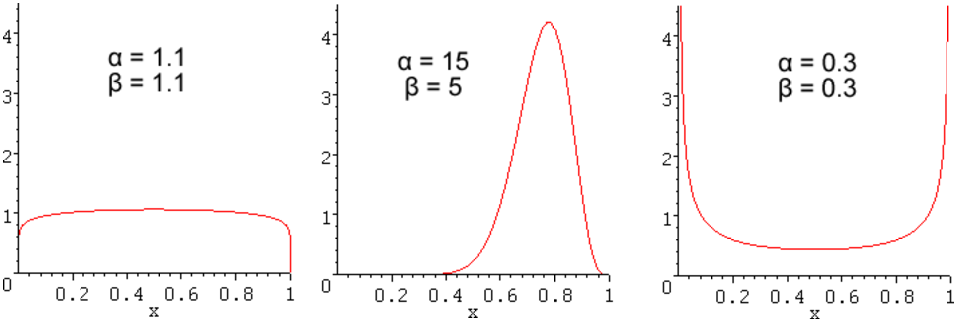
\includegraphics[scale=0.65]{BetaDistributions.png}
%\caption{some shapes of the Beta distribution}
%\end{figure}

%\begin{enumerate}
%\item The first graph shows an almost uniform distribution, which represents a high amount of uncertainty.
%\item The second graph is unimodal.
%\item The third graph shows a U shape.  As \S\ref{sec:unifying-P(Z)} shows, it is useful for representing variables with ``binary'' character.
%\end{enumerate}

Some characteristics of its shape:\\
1. If $a > 1$ and $b > 1$ the shape is unimodal with the mode at $x = \frac{a - 1}{a + b - 2}$.\\
2. If $a < 1$ and $b < 1$ it is a U shape with an anti-mode at the same point, $x = \frac{a - 1}{a + b - 2}$.\\
3. If $a = b = 1$ it is the uniform distribution.\\
4. If $a = 1$ (respectively $b = 1$) then f(x) has a finite non-zero value at $x = 0$ (respectively at $x = 1$).\\
5. If $(a-1)(b-1) \leq 0$ it is J or reverse-J shaped, without a mode or anti-mode.\\
6. If $a = b$ the pdf becomes symmetric about $x = \frac{1}{2}$.\\
7. If $b > a$ the pdf is skewed to the right, and vice versa.

%The multi-variable version of the Beta distribution is the Dirichlet distribution.

It is very useful that the mean $\mu$ and variance $v$ are given by:
\begin{eqnarray}
 \mu &=& \frac{a}{a + b} \\
 v   &=& \frac{ab}{(a + b)^2 (a + b + 1)}
\end{eqnarray}
and their inverse can be solved (by Maple) to give:
\begin{eqnarray}
 a &=& \frac{m(v + m^2 - m)}{v} \\
 b &=& \frac{(v + m^2 -m)(m - 1)}{v}
\end{eqnarray}
From the above it can be seen that the maximum variance occurs at:
$$ v_{max} = m - m^2 $$
at which point the probability mass is entirely at the poles.

Further discussion about how the Beta distribution represents $\mathcal{P(Z)}$ variables is in \S\ref{sec:unifying-P(Z)}.

\section{Causality}

Three recent books that tackle the problem of causality from an AI perspective are: \citep*{Shafer1996}, \citep*{Pearl2000}, and \citep*{Williamson2005}.  There is also a comprehensive reference \citep*{Beebee2009}.

As \citep*{Koller2009}, Ch 21, explains:  We know that a Bayesian network is directed, but the direction of the arrows do not have to be meaningful.  They can even be anti-temporal.  On the other hand, it is common wisdom that a ``good'' BN structure should correspond to causality, in that an edge $X \rightarrow Y$ often suggests that $X$ ``causes'' $Y$, either directly or indirectly.  Bayesian networks with a causal structure tends to be sparser and more natural.  However, as long as the network structure is capable of representing the underlying joint distribution correctly, the answers that we obtain to probabilistic queries are the same, regardless of whether the network structure is causal or not.


It seems that causal relations cannot be captured simply by probabilistic relations but require some form of inductive algorithm to obtain, such as the IC (for ``inductive causality'') algorithm proposed by \citep*{Pearl2000}.

\underconst

\section{First order logic and Bayesian networks}
\label{sec:FOL-BN}

Early developments in Bayesian network are mainly propositional, which means that each node in a network represents a proposition without variables, such as ``the fact that the alarm sounded''.  It has long been recognized that ``lifting'' Bayesian networks to first order is necessary for AI to be able to deal with open domains where \emph{relations} can be defined over many \emph{objects}.

\begin{figure}[H]
\centering
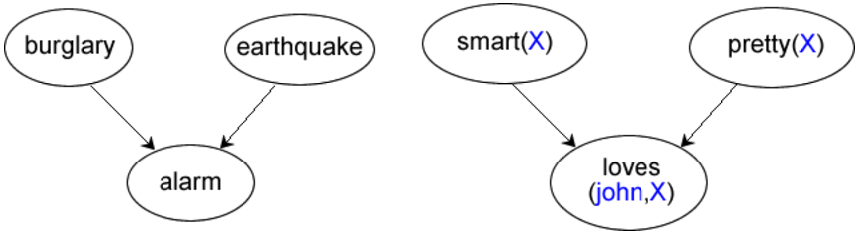
\includegraphics[scale=0.75]{FirstOrderBayesNet.png}
\caption{propositional vs first-order Bayesian networks}
\end{figure}

One key idea in first-order Bayesian networks is the method of Knowledge-Based Model Construction (KBMC), first developed by \citep*{Wellman1992} and \citep*{Haddawy1994}.  The idea is to store a knowledgebase of first-order rules that can be used to construct propositional Bayesian networks on demand.  When a query is asked, a Bayesian network is generated on-the-fly to answer the query.  This idea helps us think of the first-order case in terms of the propositional case (though it may not be the most efficient implementation in practice).

Also, I have chosen the ``directed'' approach based on Bayesian networks, versus the ``undirected'' approach based on Markov networks (eg \citep*{Domingos2007}'s Markov Logic Network (MLN)).  It seems that the directed approach is more intuitive, in which probabilistic conditionals are used to represent \emph{causal} relations.

See the book \citep*{Getoor2007} for a collection of first-order probabilistic logic approaches.

{\bfseries Some first-order probabilistic logics:}

\citep*{Kersting2000}'s Bayesian Logic Program (BLP)

\citep*{Laskey2006}'s Multi-Entity Bayesian Network (MEBN)

\citep*{Getoor2007a}'s Probabilistic Relational Model (PRM)

\citep*{Milch2007}'s Bayesian Logic (BLOG)

{\bfseries Other first-order probabilistic logics I have not looked into:}

\citep*{Sato1997}'s PRISM

\citep*{Muggleton1996}'s Stochastic Logic Program (SLP)

\citep*{Jaeger1997}'s Relational Bayesian Network (RBN), etc...

\section{Classical logic must give way to Bayesian logic}
\label{sec:P-and-ClassicalLogic}

Now we examine the relation between Bayesian networks and classical logic.

\subsection{Classical implication is ``out''}
The notion of implication in classical logic is no longer applicable in a probabilistic setting.  To see why, consider the classical equivalence of implication\\
\hspace*{1cm} $ A \rightarrow B \equiv \neg A \vee B $\\
and if we try to calculate the probability truth value of this statement we get\\
\hspace*{1cm} $ p = P( \neg A \vee B ) = P(\neg A) + P(B) - P(B|\neg A) P(\neg A) $\\
\hspace*{1cm} = $ 1 - P(A) + P(B|A) P(A) $\\
using 3 basic rules of probabilities:\\
\hspace*{1cm} $ P(X \vee Y) \equiv P(X) + P(Y) - P(X \wedge Y) $  (regardless of whether X,Y are independent)\\
\hspace*{1cm} $ P(X \wedge Y) \equiv P(Y|X)P(X) $\\
\hspace*{1cm} $ P(X) \equiv P(X|Y)P(Y) + P(X|\neg Y)P(\neg Y) $.

Now we have 4 things:\\
\hspace*{1cm} 1.  $ P(A) $\\
\hspace*{1cm} 2.  $ P(B) $\\
\hspace*{1cm} 3.  $ P(B|A) $\\
\hspace*{1cm} 4.  $ P(A \rightarrow B) = P(\neg A \vee B) = p $\\
but they cannot be fixed independently of each other: if we fix any 3 the 4th will also be fixed.

What is the problem here?  The classical implication ``$A \rightarrow B$'' serves a function \textit{similar} to the probabilistic conditional $P(B|A)$, but they constrain probabilities in slightly different ways, so they conflict with each other.  If we keep both copies of \#3 and \#4 in our KB, and apply machine learning to learn their truth values, the values may fail to converge.  It seems that classical implication is only \emph{accidentally} equivalent to $\neg A \vee B$ when things are binary.  In the probabilistic setting, we should jettison the binary implication in favor of the probabilistic conditional.

Adding probabilities to binary logic in a direct way (ie, using the binary material implication instead of $P(B|A)$) will result in very awkward inference algorithms (cf \citep*{Ng1992}, \citep*{Nilsson1986}) that require setting up sets of inequalities for probability bounds.  The result is so awkward that I think for all practical purposes this formulation can be said to be wrong.  The Bayesian network formulation (using conditional probabilities $P(B|A)$) should be preferred.

\textbf{Translating classical logic to Bayesian networks.}  (Note:  this translation is inexact but it preserves the intended meaning informally.)  First, we can translate a first-order KB into Horn form.  This is generally impossible, since Horn logic is a strict subset of first-order logic, but it can be done if we compile the knowledgebase into a pseudo-Horn form and use a special inference algorithm (this is done in \citep*{Stickel1988}).  A Horn formula (which is equivalent to a Prolog statement) having the form:\\
\hspace*{1cm} \texttt{A :- B, C, D, ...}\\
would corresponds to:\\
\hspace*{1cm} $ P(A | B, C, D, ...) = p $\\
in a Bayesian network.  This approach is also adopted by BLP, MEBN, BLOG, and PRM (see \S\ref{sec:FOL-BN}).

\subsection{The probabilistic quantifier ``$\#$''}
\label{sec:probabilistic-quantifier}

In addition to the classical quantifiers $\forall$ (``for all'') and $\exists$ (``exists''), we can introduce a probabilistic quantifier $\#$ (``for some'').  It returns as truth value the probability of the quantified statement.

For example, the truth value of:\\
\hspace*{1cm} \formula{\#x. tall(x)} \hspace*{5cm} ``Some x's are tall''\\
can be defined as:\\
$$ \frac{|\{ x | tall(x) \}|}{| \mbox{reference class of } x |} $$

Notice that the reference class of $x$ cannot be read from the formula above; it must be specified by the \textbf{type} of $x$, such as:\\
\hspace*{1cm} \formula{\#x:human. tall(x)}.

How can the computer know the sizes of these sets?  It seems that it has to keep a record of the sizes every time a new fact is encountered.  For example:\\
When \formula{tall(john:human)} enters the sensory stream, we should note that \formula{john} belongs to the classes \formula{chinese}, \formula{male}, \formula{human}, \formula{organism}, etc.  Each of these reference classes remembers its average tallness (stored as a distribution with its mean and variance, and a confidence, which gives the size of its support).  These records will be updated according as John's tallness compares to the distributions.

In other words, for each property (ie, predicate) we have to record the distributions for (at least) the \textit{typical classes that the predicate applies to}.

\section{Interval-valued probabilities}
\label{sec:intervalP}

Sometimes, Bayesian networks fail to reproduce analogous results in classical logic unless we use interval probabilities.  Consider this example:
\begin{quote}
\emph{China and the US are in conflict. If John sides with the US, he'll be a traitor. If he sides with China, he'll be a loser. Either way, John will be miserable.}
\end{quote}

We can express the premises as conditional probabilities:\\
\hspace*{1cm} $P(\mbox{miserable} \,|\, \mbox{traitor} ) = 0.9$ \\
\hspace*{1cm} $P(\mbox{miserable} \,|\, \neg\mbox{traitor} ) = 0.8$ \\
and we want to query the probability $P(\mbox{miserable})$, but it is unknown whether John is a traitor or a patriot.

This example is exactly analogous to the ``resolution rule'' in classical logic.  The classical inference step is:

\hspace*{1cm} traitor $\rightarrow$ miserable\\
\hspace*{1cm} $\neg$ traitor $\rightarrow$ miserable\\
\hspace*{1cm} --------------------------------\\
\hspace*{1cm} miserable

If we construct a Bayesian network we will have the following CPT (conditional probability table):\\
\hspace*{1cm} \begin{tabular}{|l|l|} \hline
\textbf{traitor} & \textbf{miserable}\\ \hline
true             & 0.9\\
false            & 0.8\\ \hline
\end{tabular}

but we cannot evaluate $P(\mbox{miserable})$ since $P(\mbox{traitor})$ is not known.  This is a problem with point-valued Bayesian networks: \emph{they fail to draw some analogous conclusions of classical logic}.

However, according to probability theory:\\
\hspace*{1cm} $ P(A) = P(A | B) P(B) + P(A | \neg B) P(\neg B) $

Therefore:\\
\hspace*{1cm} $ P(\mbox{miserable}) = P(\mbox{miserable} \,|\, \mbox{traitor}) P(\mbox{traitor}) + P(\mbox{miserable} \,|\, \neg\mbox{traitor}) P(\neg\mbox{traitor}) $\\
\hspace*{1cm} $= 0.9 P(\mbox{traitor}) + 0.8 P(\neg\mbox{traitor}) $\\
\hspace*{1cm} $= 0.9 p + 0.8 (1 - p) $\\
\hspace*{1cm} $= 0.8 + 0.1 p $\\
\hspace*{1cm} $= [0.8, 0.9] $

In other words, if we allow the use of interval probability, we can infer that $P(\mbox{miserable}) = [0.8, 0.9]$ even when we assume that $P(\mbox{traitor}) = [0,1]$ (ie, unknown). Thus we obtain a result analogous to classical resolution.

We need a Bayesian network inference algorithm that can handle this type of deduction, but first we consider an important simplification in the next section.  The final algorithm will be given in \S\ref{sec:P-inference}.

\section{Why point-valued probability is sufficient for AGI}
\label{sec:PointValued}

In my opinion, second-order probability (such as interval probability or the indefinite probability developed by \citep*{Walley1991} and used in \citep*{Goertzel2008}) is an overkill for AGI.  It makes the deduction algorithm very complex, and since the machine learning algorithm is based on deduction and is \textit{even more} complex, the latter problem becomes practically impossible to solve in those settings.  So we must make the deduction algorithm as simple as possible.  Therefore I suggest using only point-valued probability.

In \S\ref{sec:intervalP} I showed that interval probability is needed for some inference steps.  That means the probability P itself is uncertain, and it lies in an interval.  The \emph{exact} algorithm for interval-probability inference requires us to set up the bounds of various probabilities and then invoke linear programming to solve for the probability bounds of the query variable (This method was first outlined by \citep*{Boole1854} and then developed by \citep*{Hailperin1965}, \citep*{Nilsson1986}, \citep*{Ng1992} et al. Recently \citep*{Hansen2000}, \citep*{Jaumard2006} developed faster algorithms for it, but still, the complexity of these algorithms is too much to handle if we want to design learning algorithms based on them.)

What I propose is that whenever we obtain an interval P value, we should convert it to a point value by \emph{taking the mid-point of the interval}.\footnote{We still need inference algorithms that can handle intervals as demonstrated in \S\ref{sec:intervalP}, but the intervals will be instantly converted to point-values after each step. This reduces complexity greatly.}

For example, John may be unable to decide whether the president is smart or dumb.  He may ascribe $P = [0.2,0.8]$ to the atom $smart(president)$.  According to my scheme, he can use \[ P = (0.2 + 0.8) / 2 = 0.5 \] as a compromise.  This is like saying ``there's 50-50 chance''.  Is this approximation too bad?  It seems that many people think like this anyway.  I'd be surprised if the human brain maintains 2nd-order probabilities internally.

Moreover, the exact values of P often do not affect our behavior that much.  There is evidence that taking the centroid (the center of mass of a belief distribution) can yield reasonably good results in second-order probabilistic decision-making (\citep*{Sundgren2006}).  Also, \citep*{Bier1993} shows that there are broad classes of utility functions for which uncertainty is irrelevant under expected utility theory, and only mean values are significant.  \{ TO-DO:  There is hand-waving here. \}

Maybe in a much more advanced AGI, we would want 2nd-order precision, but that seems not to be the right priority now.  It may be more effective for an AGI to improve its decisions by:\\
\hspace*{1cm} 1. considering more factors;\\
\hspace*{1cm} 2. updating probabilities using more evidence;\\
\hspace*{1cm} 3. refining explanations (causal relations);  etc.

Using point-valued probabilities (without knowing their error) is not such a big sin, if we compare this with what we do in fuzzy logic all the time.  A fuzzy statement such as:\\
\hspace*{1cm} ``John is fairly tall''\\
is often represented simply by:\\
\hspace*{1cm} tall(john) \hspace{0.5cm} $z = 0.7$\\
which is analogous to representing the probabilistic statement\\
\hspace*{1cm} ``John is usually punctual''\\
with a point-valued probability:\\
\hspace*{1cm} punctual(john) \hspace{0.5cm} $p = 0.8$.

If fuzziness is a more fundamental phenomenon in our knowledge representation, we should be making more fuss about fuzziness than probabilities.  It seems that we ascribe more ``prestige'' to probability theory merely because of psychological reasons.

\section{Probabilistic AND and OR}
\label{sec:P-and-or}

Specifying the CPT (conditional probability table) of a single node of a Bayesian network, if the node has $n$ parents, would require $2^n$ entries.  The ``noisy'' AND and OR gates are designed to simplify this by reducing the number of independent entries to $n$.  The interpretation of the noisy OR gate is that each parent variable $X$ is associated with an ``inhibition probability'', $q$ (\citep*{Pearl1988} p184-187 or \citep*{Russell2003} p500-501).  This is the textbook definition of noisy OR (and I created noisy AND by applying DeMorgan's law\footnote{That is, to require $\overline{X_1 \curlyvee X_2} \equiv \overline{X_1} \curlywedge \overline{X_2}$ and $\overline{X_1 \curlywedge X_2} \equiv \overline{X_1} \curlyvee \overline{X_2}$ }):

\hspace*{1cm} \begin{tabular}{|l|l||l||l|} \hline
\multicolumn{2}{|c||}{} & {\textbf{noisy AND}}           & {\textbf{noisy OR}}\\ \hline
$X_1$ & $X_2$           & $X_1 \Pand X_2$          & $ X_1 \Por X_2 $\\ \hline
0     & 0               & $ 1 ? $                        & $ 0 $\\
0     & 1               & $ 1 - q_1 ? $                  & $ 1 - q_1 $\\
1     & 0               & $ 1 - q_2 ? $                  & $ 1 - q_2 $\\
1     & 1               & $ 1 - q_1 - q_2 + q_1 q_2 ? $  & $ 1 - q_1 q_2 $\\ \hline
\end{tabular}

It seem that this definition of noisy AND is problematic (for example, the ``1'' there should be close to 0).

\{ TO-DO:  Abram Demski pointed out that the textbook definition of noisy-OR is actually OK and there is no need to invent a new one. \}

Anyway, I defined my version of ``probabilistic'' AND and OR so that they obey DeMorgan's laws.  Each variable is attached with a ``causal strength'' $c \in [0,1]$, such that when $c \rightarrow 1$ they reduce to classical AND and OR.

It is better to write the complement $(1 - c)$ as superscript.  So the pair $c_l, (1 - c_l)$ is written as $\vec{c}^i = c_i^0, c_i^1$.  In this notation my definitions can be expressed simply as:
\begin{eqnarray}
 X_1 \Pand X_2 & = & \sum_{i j} \; ( \vec{c}^i_1 \, \vec{c}^j_2 \, \vec{x}^i_1 \, \vec{x}^j_2 ) \\
 X_1 \Por  X_2 & = & \sum_{i j} \; ( ( \vec{c}^i_1 + \vec{c}^j_2 - \vec{c}^i_1 \, \vec{c}^j_2 ) \; \vec{x}^i_1 \, \vec{x}^j_2 )
\end{eqnarray}
which can be easily generalized to $n > 2$.  When expanded, they yield the following table:

\hspace*{1cm} \begin{tabular}{|l|l||l||l|}
\hline
\multicolumn{2}{|c||}{} & {\textbf{probabilistic AND}} & {\textbf{probabilistic OR}}\\
\hline
%\rule[-3mm]{0mm}{8mm}
$X_1$ & $X_2$ & $X_1 \Pand X_2$          & $X_1 \Por X_2$\\ \hline
0     & 0     & $(1-c_1) (1-c_2)$        & $1 - c_1 c_2$\\
0     & 1     & $(1-c_1) \; c_2$         & $1 - c_1 + c_1 c_2$\\
1     & 0     & $c_1 \; (1-c_2)$         & $1 - c_2 + c_1 c_2$\\
1     & 1     & $c_1 \; c_2$             & $c_1 + c_2 - c_1 c_2$\\
\hline
\end{tabular}
\parbox{8cm}{\begin{equation}
\label{eqn:probabilistic-AND-OR}
\end{equation}}

A CPT can be defined by a combination of probabilistic AND-OR's:
\begin{equation}
X_0 := \bigPor_i \; \bigPand_j \; X_{ij}
\end{equation}
where the $X_{ij}$'s are parents of the node $X_0$ in the Bayesian network.

Notice that in the above equation, each connective is associated with a pair of c parameters, so the actual equation is:
\begin{equation}
X_0 := \bigPor_i \; \bigPand_j \; X_{ij};c_{ij} \; = \bigPor \; \{ X_{11};c_{11} \Pand X_{12};c_{12} \Pand \cdots, X_{21};c_{21} \Pand X_{22};c_{22} \Pand \cdots, \; \cdots \}
\end{equation}
It can be verified that \emph{association} holds as in classical logic, ie:
\begin{eqnarray}
(A \Pand B) \Pand C & = & A \Pand (B \Pand C), \\
(A \Por   B) \Por   C & = & A \Por   (B \Por   C),
\end{eqnarray}
a fact that can be exploited for efficient calculation.  This is because the CPT (conditional probability table) has size $2^n$ where $n$ is the number of variables.  But when the operator is associative, we can calculate $\bigZand_i X_i$ as $((X_1 \Zand X_2) \Zand X_3) \Zand ...$, without having to generate the full CPT.  Thus the space complexity remains constant.

It is also possible to use the trick in \S\ref{sec:unifying-AND-and-OR} to combine AND and OR with the parameter $\theta$:
\begin{equation}
X_1 \varodot X_2 = (1-\theta) (X_1 \Pand X_2) + \theta (X_1 \Por X_2)
\end{equation}

% TO-DO:  weighted noisy AND-OR may not be needed, because the weights are absorbed into the c's
